\documentclass[10pt]{beamer}

\mode<presentation>
{
  \usetheme{boxes}      % or try Darmstadt, Madrid, Warsaw, ...
  \usecolortheme{default} % or try albatross, beaver, crane, ...
  \usefonttheme{structurebold}  % or try serif, structurebold, ...
  \setbeamertemplate{navigation symbols}{}

  \setbeamertemplate{caption}[numbered]
}

\usepackage[english]{babel}
\usepackage[utf8x]{inputenc}
\usepackage{tikz}
\usepackage{graphicx}
\usepackage{float}
\usepackage{subfig}

\DeclareGraphicsExtensions{.pdf,.png,.jpeg}


\definecolor{structurColor}{RGB}{67, 98, 194}
\definecolor{HHred}{RGB}{242, 56, 90}
\definecolor{HHblue}{RGB}{52, 56, 68}
\definecolor{HHturquoise_d}{RGB}{34, 137, 165}
\definecolor{HHturquoise_m}{RGB}{54, 177, 191}
\definecolor{HHturquoise_l}{RGB}{74, 217, 217}
\definecolor{HHwhite}{RGB}{233, 241, 223}
\definecolor{HHyellow}{RGB}{253, 197, 54}
\definecolor{HHwhite2}{RGB}{250, 250, 250}
\definecolor{applegreen}{rgb}{0.55, 0.71, 0.0}
\definecolor{cadmiumorange}{rgb}{0.8, 0.33, 0.0}

\setbeamertemplate{itemize item}[ball]
\setbeamertemplate{itemize subitem}[circle]
\setbeamercolor{frametitle}{fg=structurColor}
\setbeamercolor{structure}{fg=structurColor}

\title{\textcolor{HHwhite}{Search for Higgs pair production at LHC Collider (CERN): The first measurement for Higgs potential and search for new physics}}
\subtitle{\textcolor{HHwhite}{Ph.D. thesis defence}}

\author{ 
\textcolor{HHwhite}{
{\textbf{Mohamed BELFKIR}} \\
{\and} \\
{\textit{Supervised by}} \\
{\textsf{Stephane JEZEQUEL}}
}
}
\date{}

\logo{\insertframenumber/\inserttotalframenumber}

\begin{document}
\setbeamercolor{background canvas}{bg=HHwhite2}
{
\usebackgroundtemplate{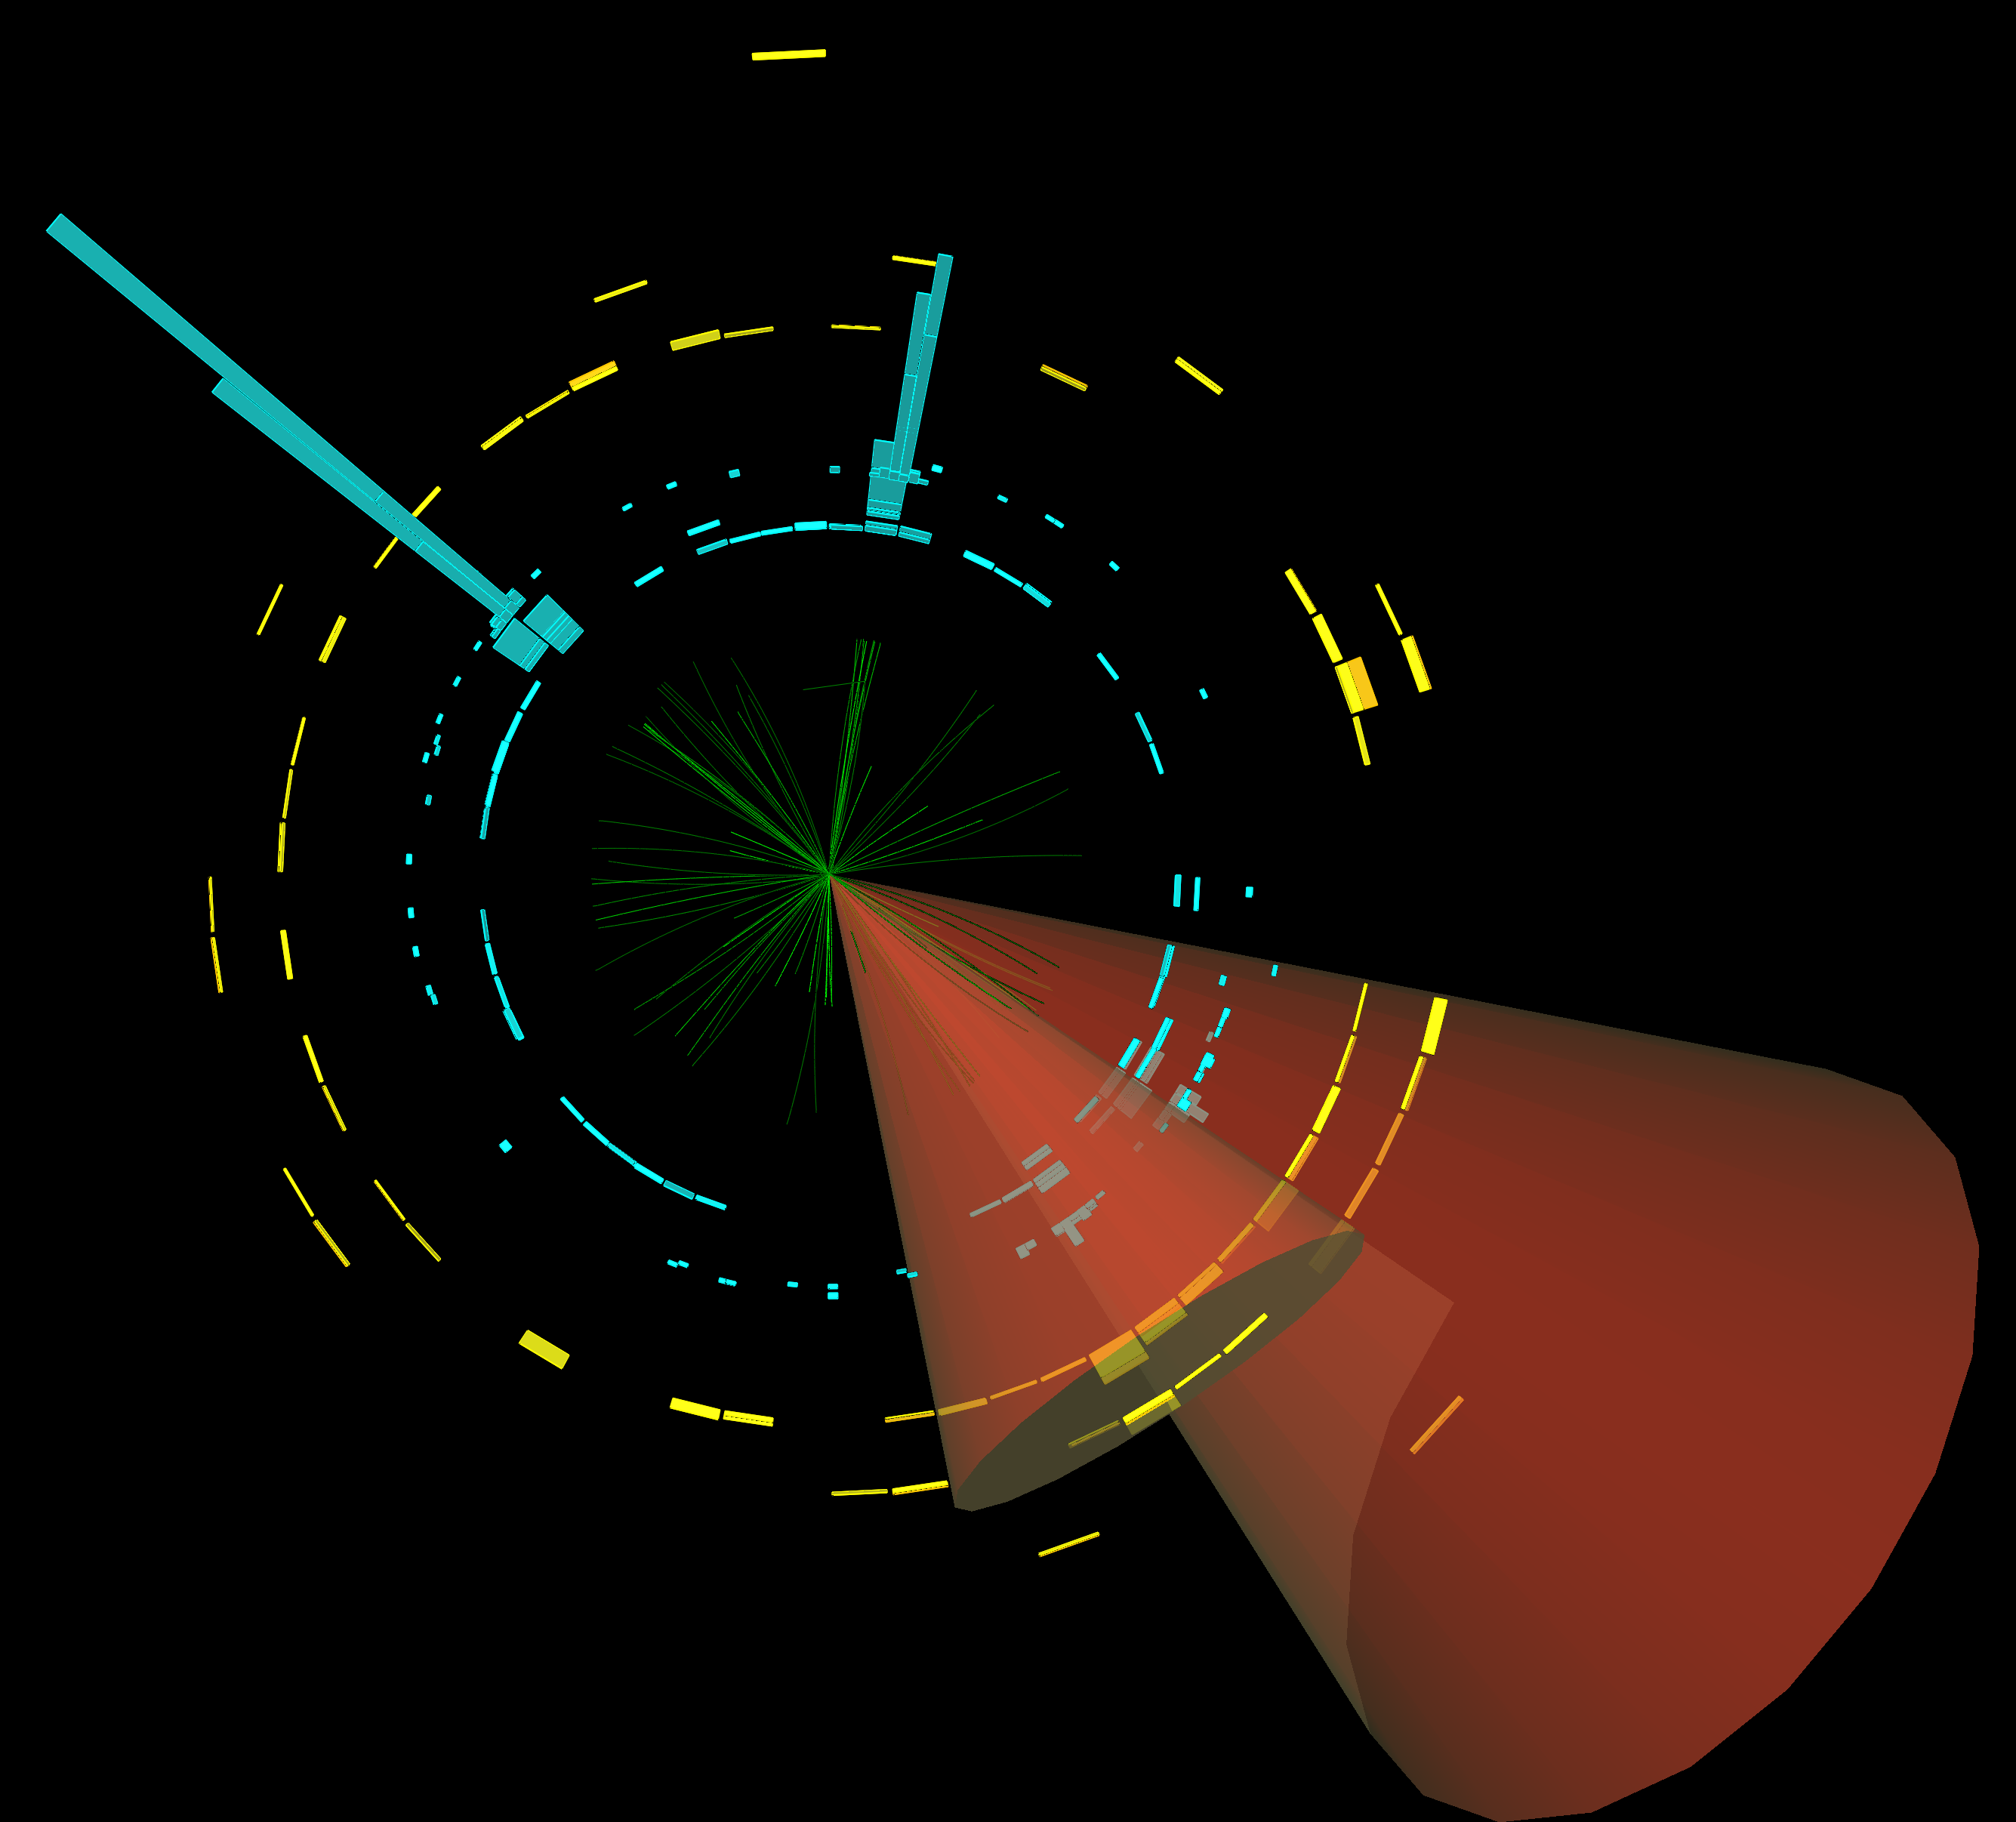
\includegraphics[width=\paperwidth]{Img/figaux_02}}
\begin{frame}
\titlepage
\end{frame}
}

\section*{Content}
\begin{frame}{Content}
\label{content}
    \tableofcontents
\end{frame}

\section{Theoretical framework}
\begin{frame}{Content}
\label{content}
    \tableofcontents[currentsection]
\end{frame}

\subsection{The Standard Model of particle physics}

\begin{frame}{The Standard Model (SM) of particle physics}

%\begin{textblock*}{5cm}(13.2cm, 3.cm) % {block width} (coords) 
%   \textbf{\textcolor{HHturquoise_d}{Strong}}
%\end{textblock*}
%\begin{textblock*}{5cm}(13.2cm, 4.2cm) % {block width} (coords) 
%   \textbf{\textcolor{HHturquoise_m}{Electromagnetic}}
%\end{textblock*}
%\begin{textblock*}{5cm}(13.2cm, 5.4cm) % {block width} (coords) 
%   \textbf{\textcolor{HHturquoise_m}{Weak}}
%\end{textblock*}

\begin{columns}
\column{0.5\textwidth}

\begin{itemize}
    \item Quantum field theory, based on the principal gauge invariance $\textcolor{HHturquoise_d}{SU(3)}\times \textcolor{HHred}{SU(2)}\times \textcolor{HHturquoise_m}{U(1)}$
    \item Unify \textbf{\textcolor{HHturquoise_d}{Strong}} and \textbf{\textcolor{HHturquoise_m}{Electro}-\textcolor{HHred}{weak}} interactions
    \item \textbf{Fermions}: matter particles
    \begin{itemize}
        \item \textbf{\textcolor{violet}{Quarks}}
        \item \textbf{\textcolor{applegreen}{Leptons}}
    \end{itemize}
    \item \textbf{\textcolor{cadmiumorange}{Gauge bosons}}: mediators of interactions
\end{itemize}    
\begin{itemize}    
    \item \textbf{\textcolor{HHyellow}{Higgs boson}}: responsible for mass generation through EWSB mechanism
    
\end{itemize}

\column{0.5\textwidth}
\begin{figure}
    \centering
    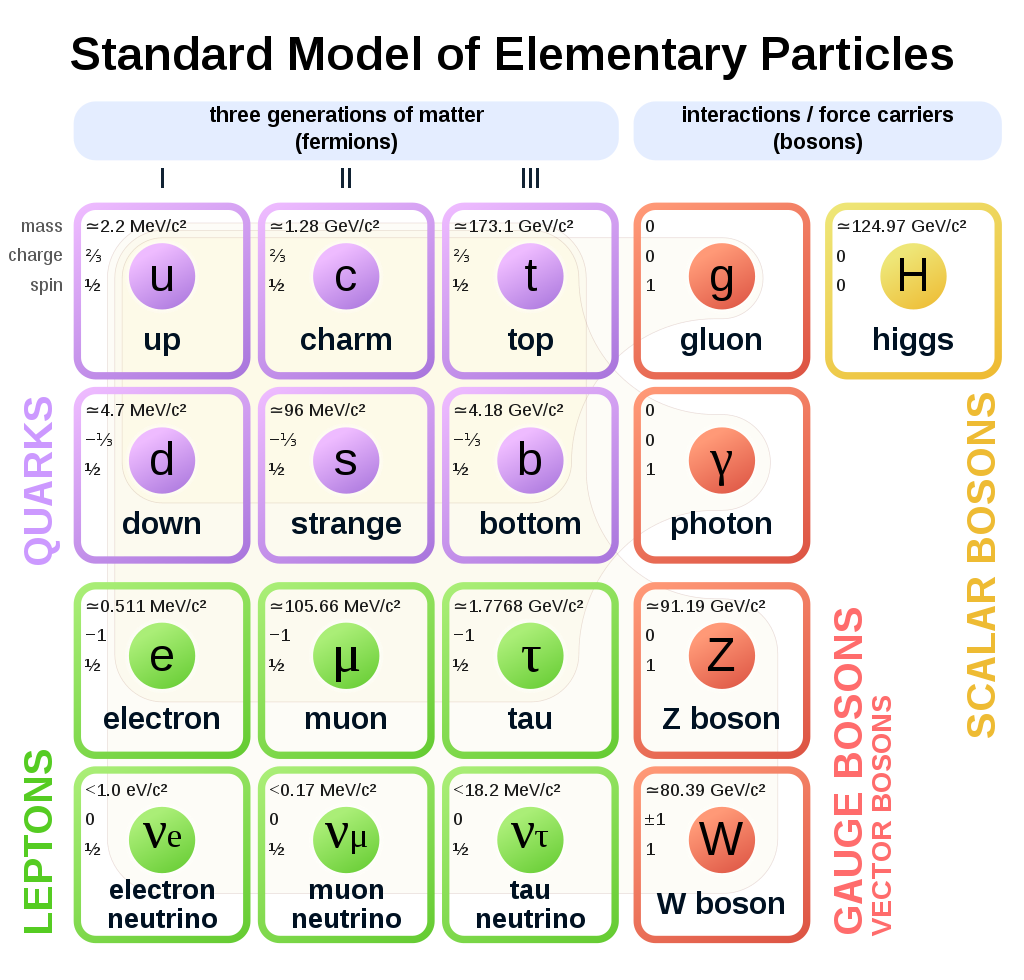
\includegraphics[width=1\textwidth]{Part1/Img/SM_particles.png}
\end{figure}
\end{columns}
\end{frame}

\begin{frame}{Electroweak Symmetry Breaking and Higgs boson}
\setbeamercovered{transparent}
\begin{textblock*}{5cm}(12.2cm, 6.5cm) % {block width} (coords) 
\visible<2>{
\begin{figure}
    \begin{overprint}
    \centering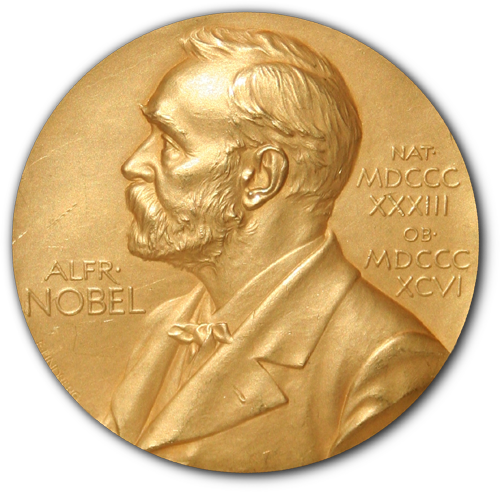
\includegraphics[width=0.2\textwidth]{Part1/Img/Nobel_Prize.png}
    \end{overprint}
\end{figure}
}
\end{textblock*}
\begin{textblock*}{5cm}(10cm, 3.9cm) % {block width} (coords) 
$\mu^2 <$ 0 $\to$ Mexican hat 
\end{textblock*}
\begin{columns}
\column{0.4\textwidth}
\begin{figure}
    \centering
    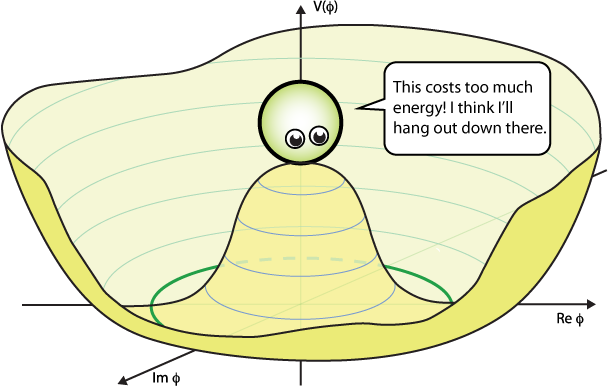
\includegraphics[width=0.8\textwidth]{Part1/Img/Higgs-Potential-lookdown.png}
\end{figure}
\visible<2>{
\begin{figure}
    \centering
    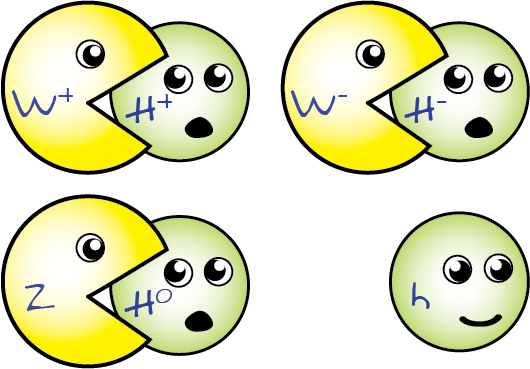
\includegraphics[width=0.8\textwidth]{Part1/Img/Goldstone-Eaten-four.png}
\end{figure}
}
\column{0.6\textwidth}
Gauge boson mass terms break gauge symmetry of SM
\begin{itemize}
    \item \textcolor{structurColor}{Brout-Englert-Higgs (1964)} include complex scalar field
    \begin{equation*}
        V(\phi^\dagger\phi) = \mu^2\phi^\dagger\phi + \lambda(\phi^\dagger\phi)^2
    \end{equation*}
    \pause
    \item Choice of the vacuum state $v$ \textbf{\textcolor{applegreen}{spontaneously breaks the symmetry}}
    \begin{itemize}
        \item Gauge bosons become massive
        \item \textbf{Higgs boson}: $m_{H}= -2\mu^2$
        \item Fermion masses: generated through Yukawa couplings
    \end{itemize}
\end{itemize}

\begin{itemize}
    \item \underline{Observed} in 2012 at LHC, $m_{H} \sim $ 125 GeV
\end{itemize}
\end{columns}
\end{frame}

\begin{frame}{Measurements of Higgs parameters}

\begin{textblock*}{5cm}(2.5cm,3.2cm) % {block width} (coords) 
   \textcolor{HHturquoise_d}{\textbf{mass}}
\end{textblock*}
\begin{textblock*}{5cm}(2cm,6.7cm) % {block width} (coords) 
   \textcolor{HHred}{\small\textbf{125.09 $\pm$ 0.24 GeV}}
\end{textblock*}

\begin{textblock*}{5cm}(7.6cm,3.2cm) % {block width} (coords) 
   \textcolor{HHturquoise_d}{\textbf{cross-section}}
\end{textblock*}
\begin{textblock*}{5cm}(12.5cm,2cm) % {block width} (coords) 
   \textcolor{HHturquoise_d}{\textbf{coupling}}
\end{textblock*}

\begin{textblock*}{5cm}(12.5cm,4cm) % {block width} (coords) 
   \small\textbf{$\sim$20\%}
\end{textblock*}

\begin{textblock*}{5cm}(14.3cm,3.2cm) % {block width} (coords) 
   \small\textbf{$<$10\%}
\end{textblock*}


\begin{figure}
    \centering
      \subfloat{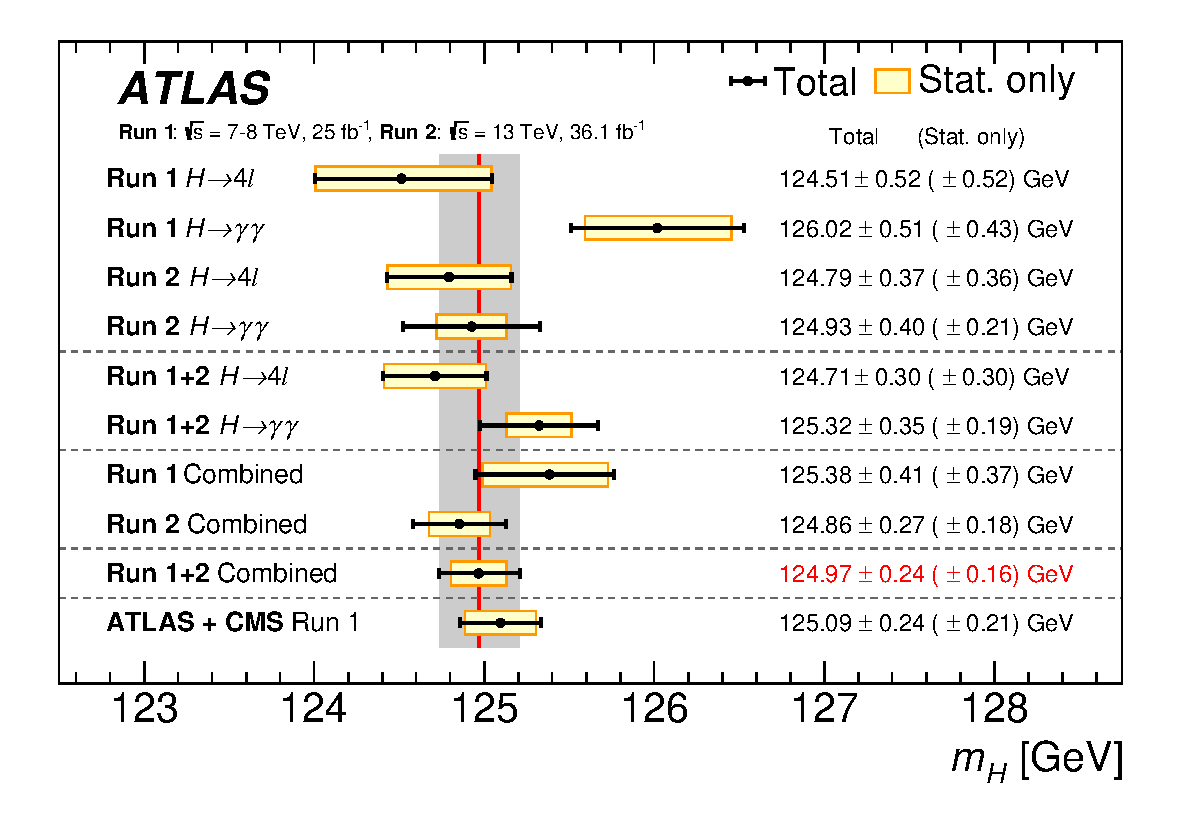
\includegraphics[width=0.35\textwidth]{Part1/Img/ATLAS_HIGGS1100_mass_Summary.pdf}}
      \subfloat{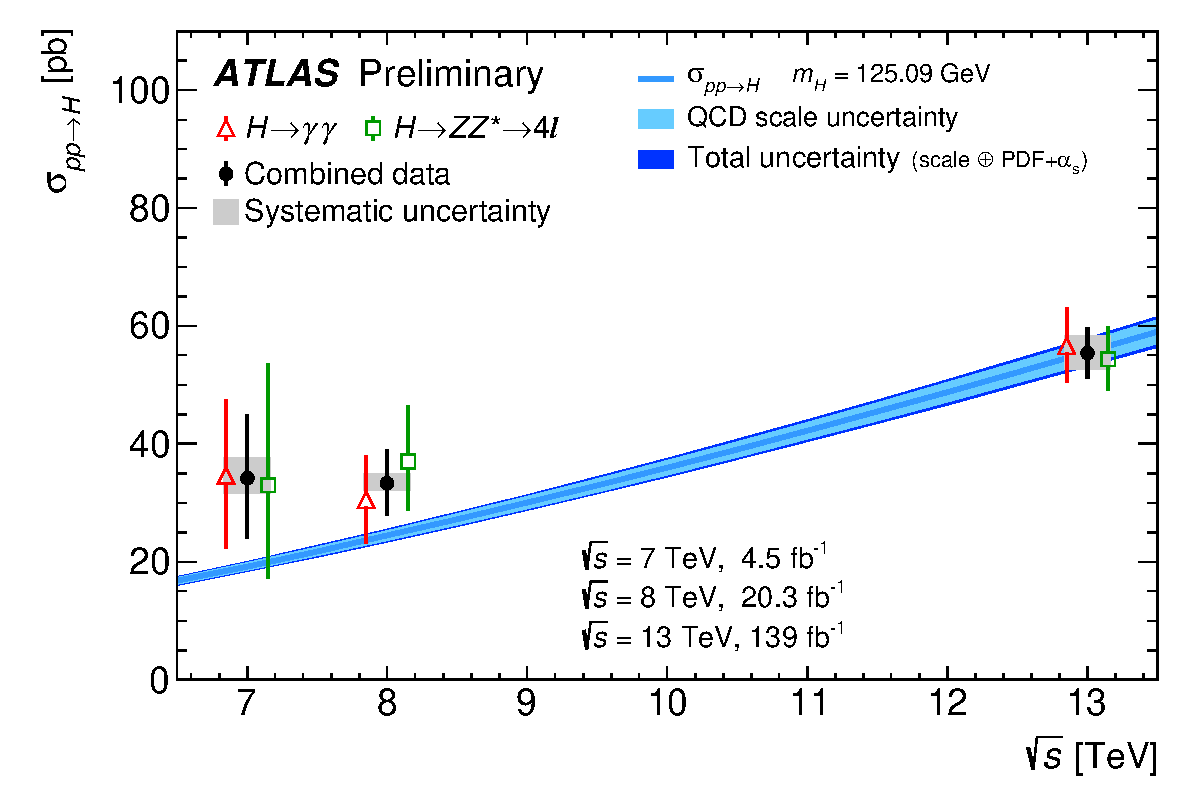
\includegraphics[width=0.35\textwidth]{Part1/Img/ATLAS_HIGGS3010_XSvsCME_Summary.pdf}}
%    \subfloat{ 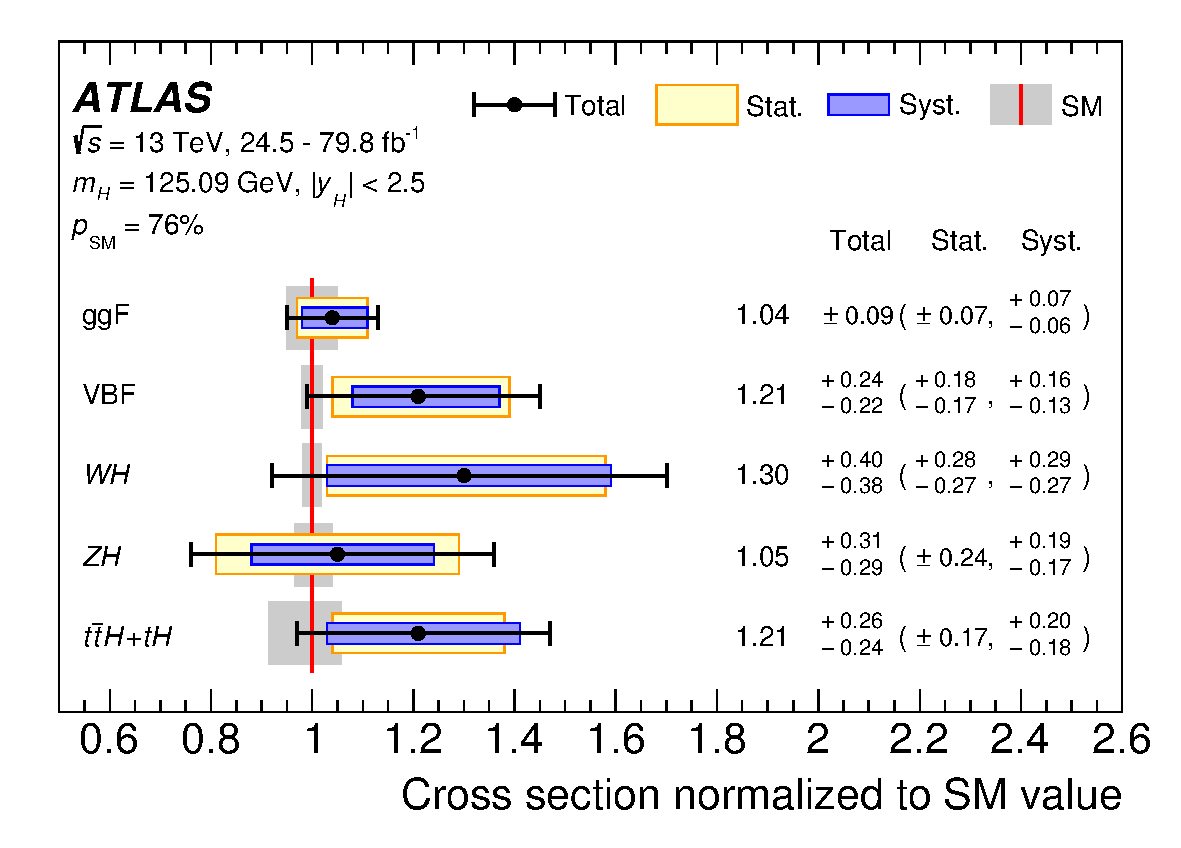
\includegraphics[width=0.5\textwidth]{Part1/Img/ATLAS_HIGGS3250_Run2XS_Summary.pdf}}
      \subfloat{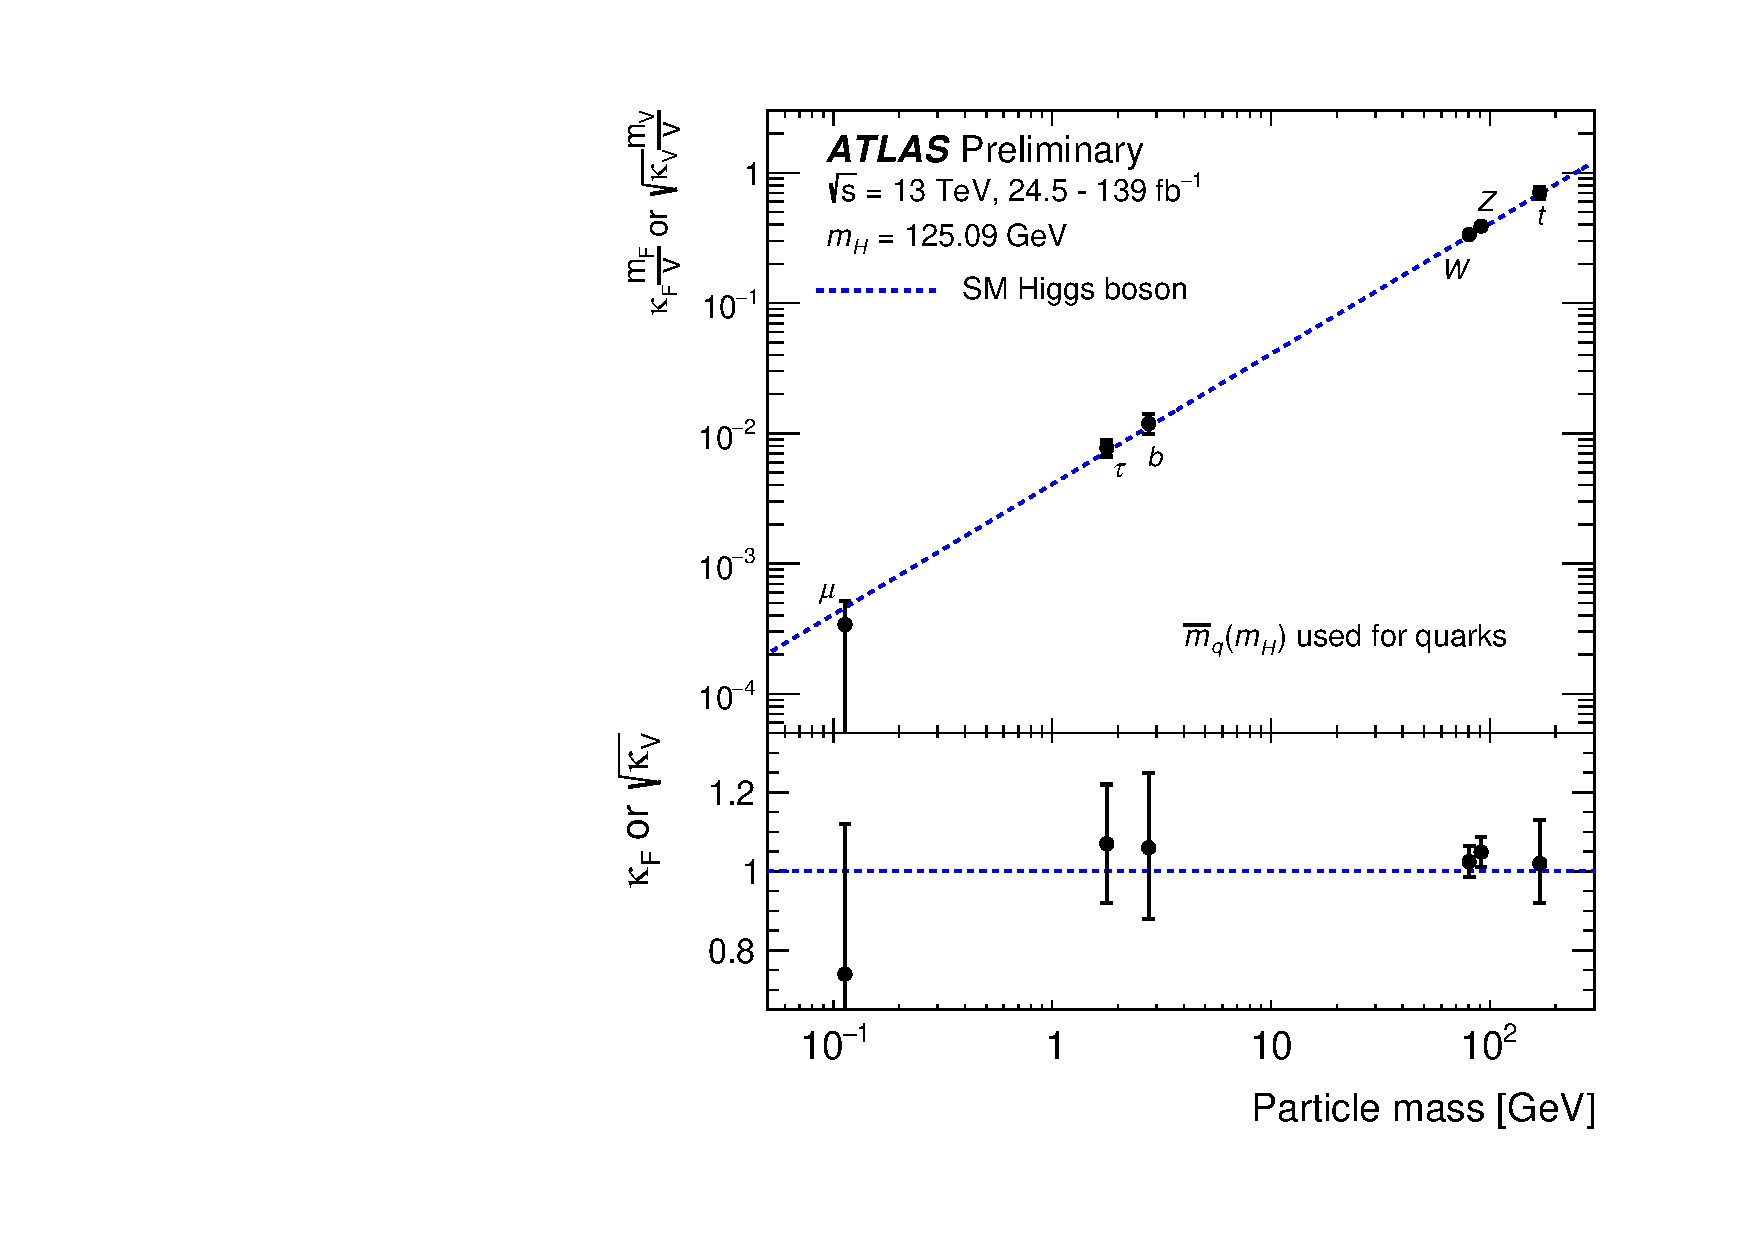
\includegraphics[width=0.35\textwidth]{Part1/Img/ATLAS_HIGGS4400_kappa_vs_mass.pdf}}
\end{figure}

\begin{itemize}
    \onslide<2>{
    \item \textcolor{HHred}{Not all, Higgs boson self-coupling still resists to physicists}
    }
\end{itemize}

\end{frame}

\subsection{Higgs boson self-coupling}

\begin{frame}{Higgs boson self-coupling}
\begin{columns}
\column{0.6\textwidth}    
\begin{itemize}
    \item \textbf{Self-coupling: \textcolor{structurColor}{Higgs boson trilinear coupling}}
    \item Controls the shape of the Higgs potential
    \begin{itemize}
        \item It is important to measure both $m_{H}$ and $\lambda$
    \end{itemize}
    \item \textbf{B}eyond \textbf{SM} (BSM) physics would impact this coupling, impact quantified as
    \begin{equation*}
       \textcolor{HHred}{\kappa_{\lambda} = \frac{\lambda}{\lambda^{SM}}}
    \end{equation*}
    \onslide<3>{
    \item Measured \underline{\textbf{directly}} with \textbf{\textcolor{HHturquoise_d}{Higgs boson pair (\textbf{HH}) production}} 
    }
\end{itemize}

\column{0.4\textwidth}  

\begin{textblock*}{5cm}(13cm,6.2cm) % {block width} (coords) 
  \visible<1>{ not accessible \\ at LHC }
\end{textblock*}

\begin{textblock*}{5cm}(14.5cm,4.2cm) % {block width} (coords) 
  \visible<2>{\textcolor{HHturquoise_d}{$\lambda=1$}} \\
  \visible<2>{\textcolor{applegreen}{$\lambda=0$}} \\
  \visible<2>{\textcolor{violet}{$\lambda=-1$}}
\end{textblock*}
\begin{equation*}
    V \supset \frac{m_{H}^2}{2}H^2 + \textcolor{HHred}{\lambda} vH^3 + \frac{\textcolor{HHred}{\lambda}}{v}H^4
\end{equation*}
\begin{equation*}
    \lambda^{SM} = \frac{m_{H}^2}{2v^2} \sim 0.13
\end{equation*}

\begin{figure}
    \begin{overprint}
    \onslide<1>\centering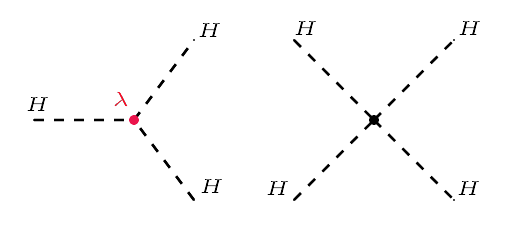
\includegraphics[width=0.9\textwidth]{Part1/Img/hhh_diagrams.png}
    \onslide<2>\centering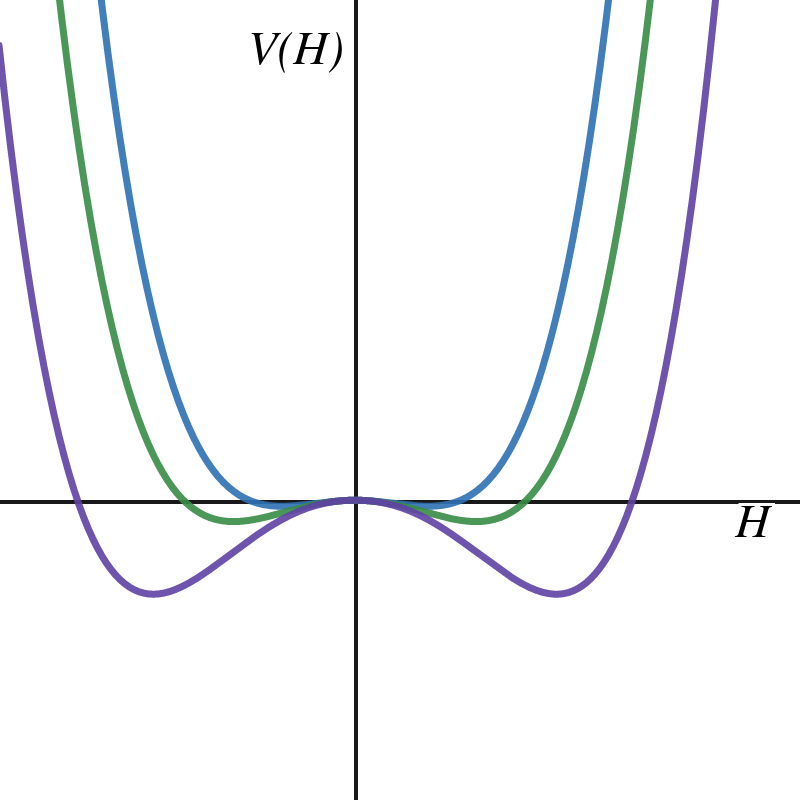
\includegraphics[width=0.8\textwidth]{Part1/Img/V_H_for_lambda.png}
    \onslide<3>\centering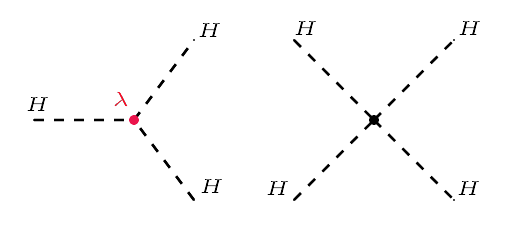
\includegraphics[width=0.9\textwidth]{Part1/Img/hhh_diagrams.png}
    \end{overprint}
\end{figure}

\end{columns}    

\end{frame}

\subsection{Higgs boson pair production}

\begin{frame}{Higgs boson pair production at the LHC}
\begin{textblock*}{5cm}(5.8cm, 1.8cm) % {block width} (coords) 
  \textcolor{black}{\textbf{Destructive interference}}
\end{textblock*}

\begin{textblock*}{5cm}(6.4cm, 2.5cm) % {block width} (coords) 
  \textcolor{black}{$\kappa_t$}
\end{textblock*}

\begin{itemize}
    \item Produced mainly via \textbf{\underline{non-resonant}} \textbf{\textcolor{HHred}{gluon-gluon Fusion}} \textbf{(ggF)} and \textbf{\textcolor{HHturquoise_d}{Vector Boson Fusion}} \textbf{(VBF)}
\end{itemize}

\begin{figure}
    \fcolorbox{HHred}{HHwhite2}{     \subfloat{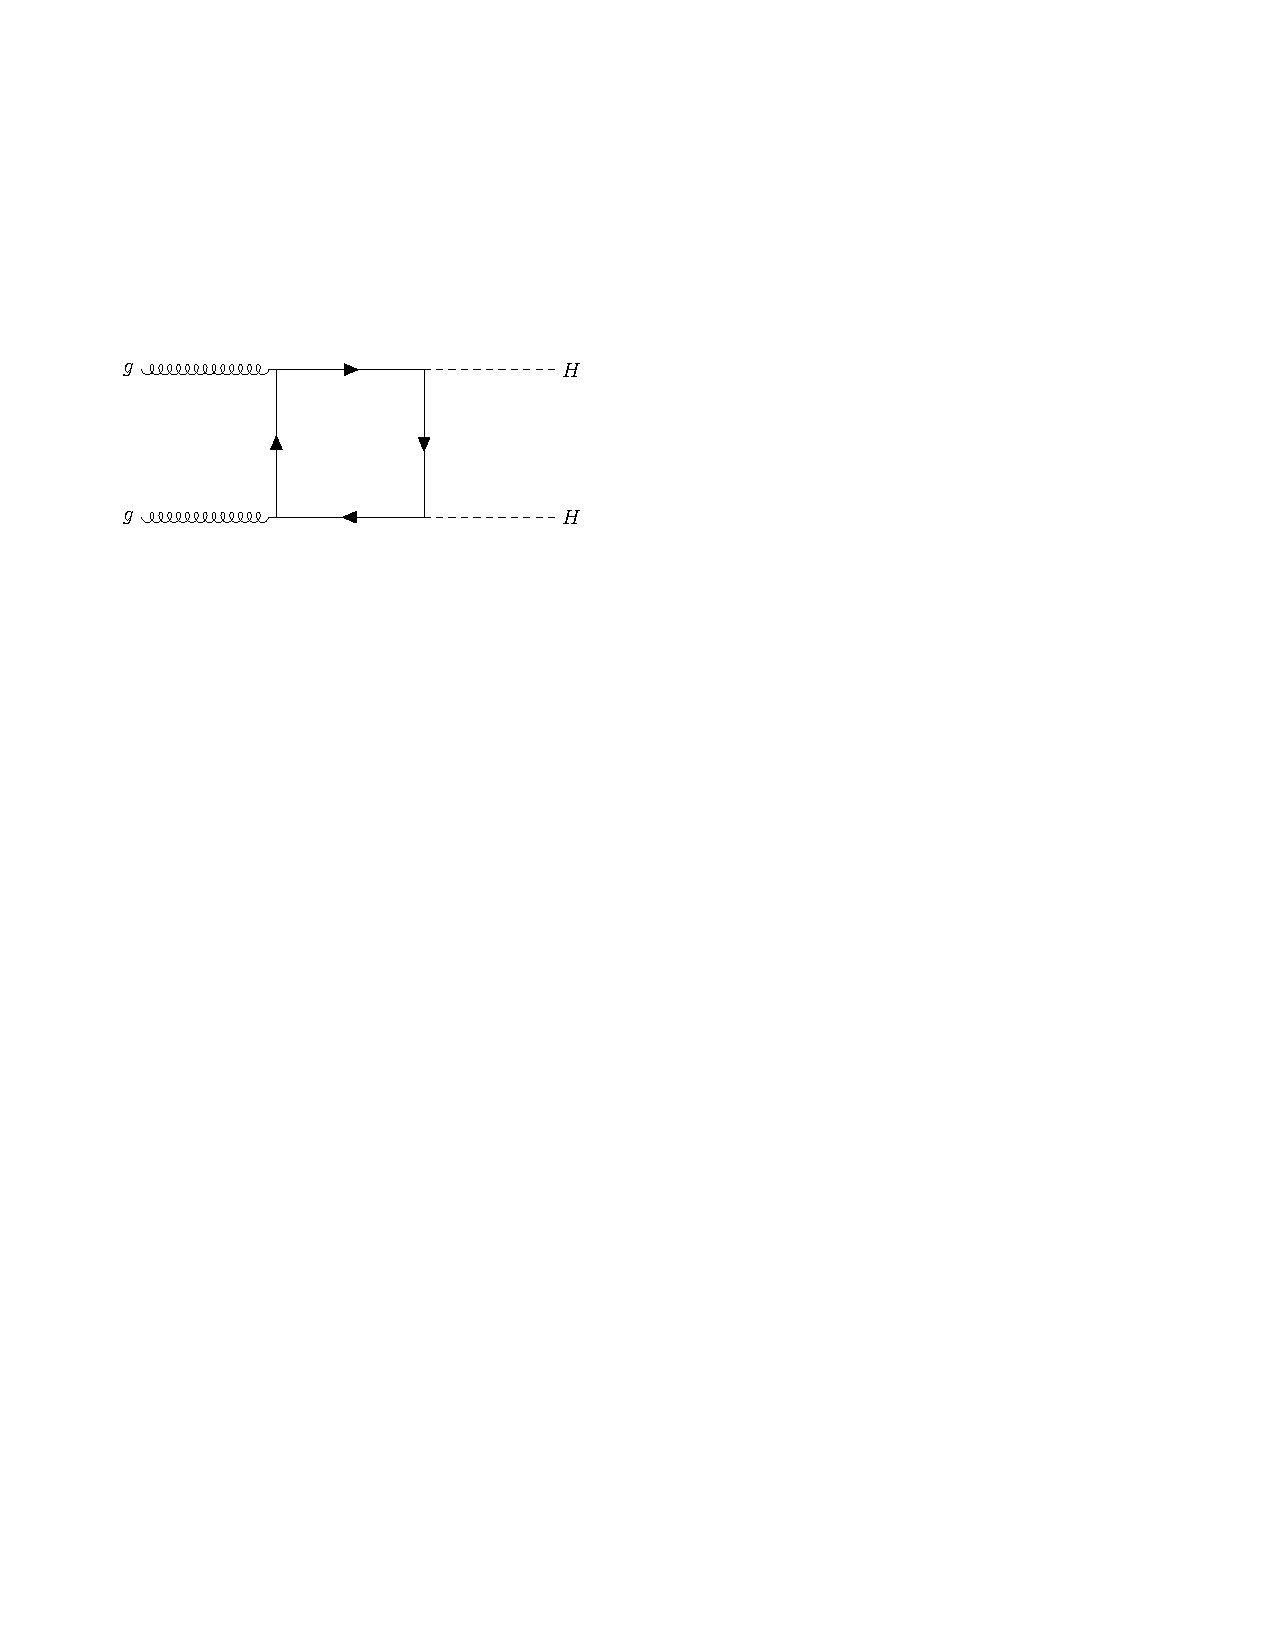
\includegraphics[width=0.3\textwidth]{Part1/Img/ggF_box.pdf}}
    \subfloat{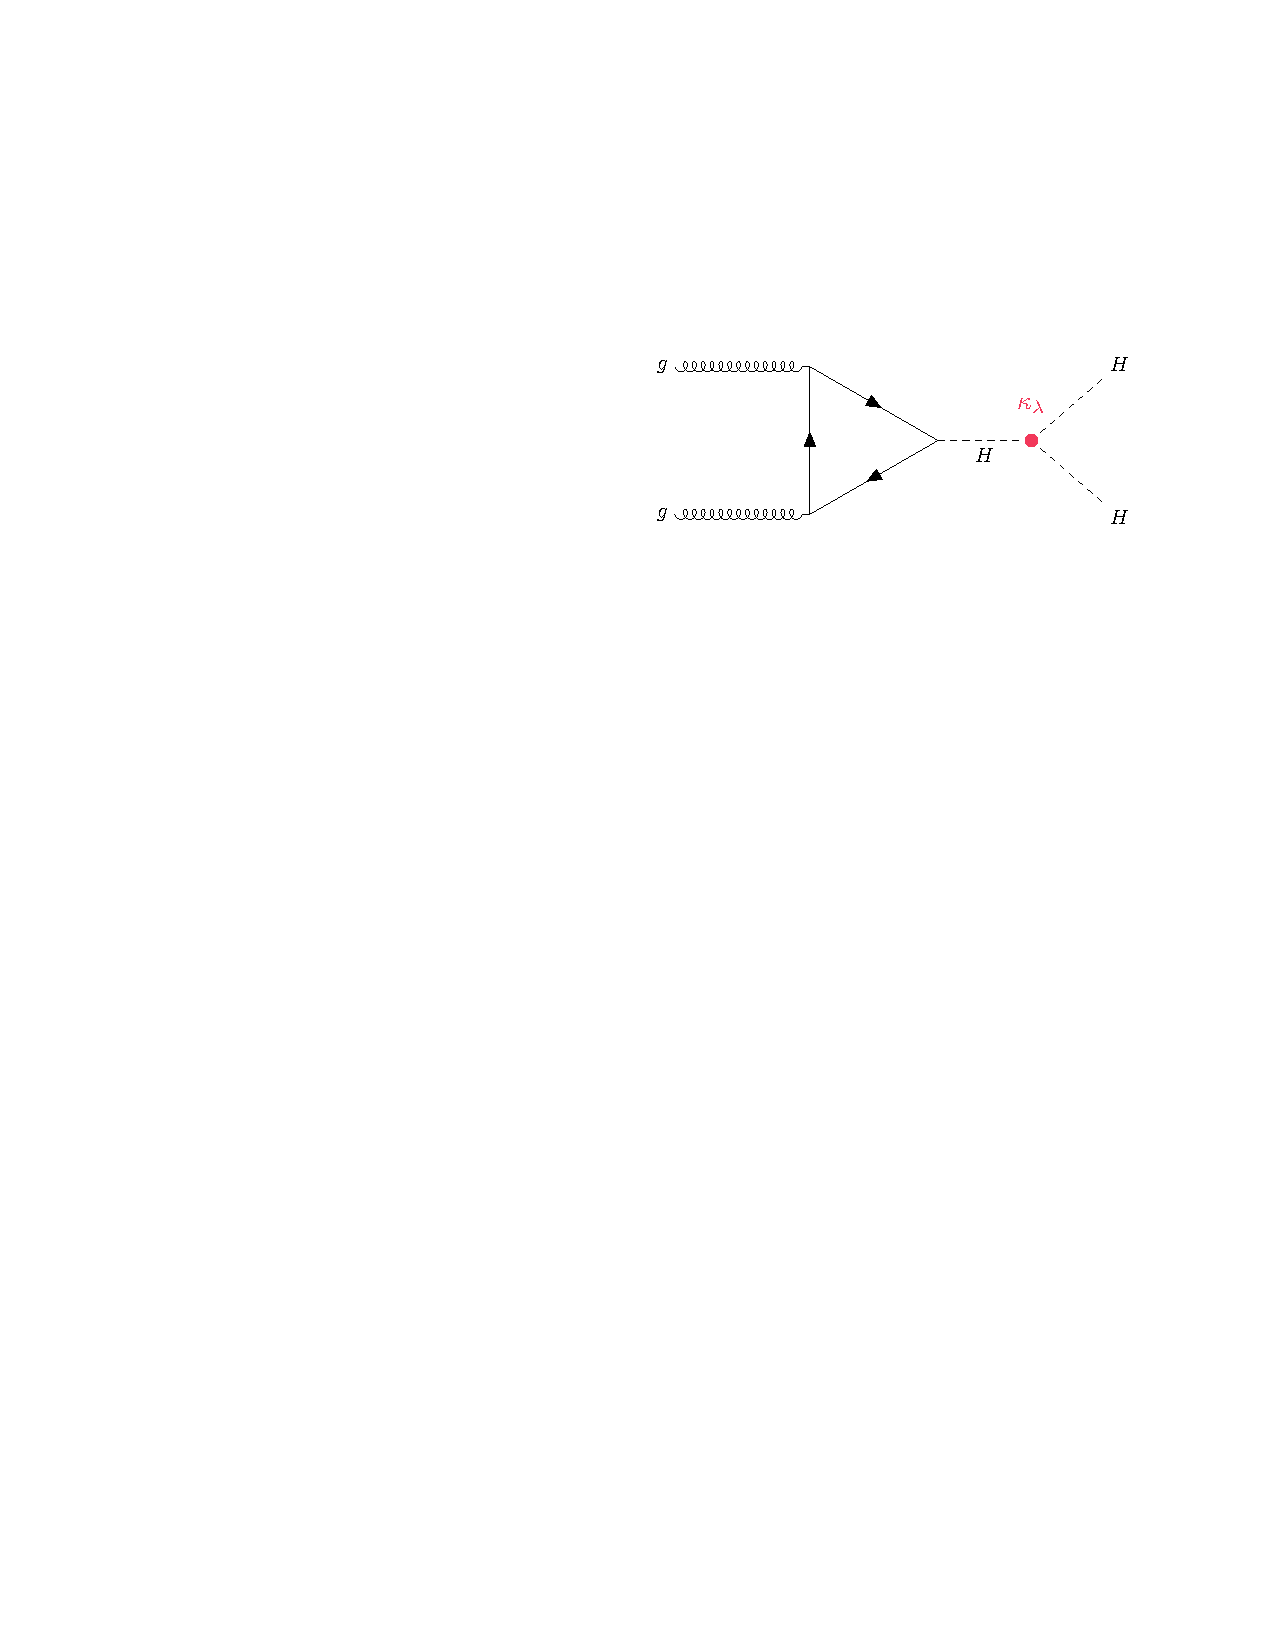
\includegraphics[width=0.3\textwidth]{Part1/Img/ggF_tri.pdf}}} \\
    \fcolorbox{HHturquoise_d}{HHwhite2}{
    \subfloat{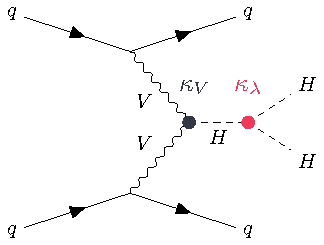
\includegraphics[width=0.2\textwidth]{Part1/Img/VBF_kvkl.pdf}}
    \subfloat{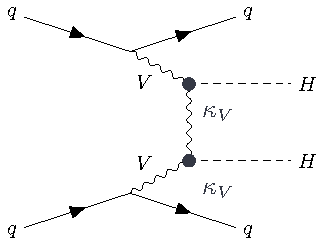
\includegraphics[width=0.2\textwidth]{Part1/Img/VBF_kvkv.pdf}}
    \subfloat{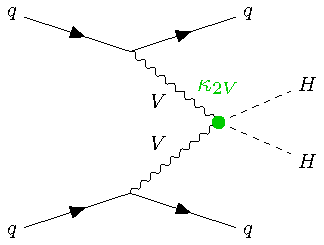
\includegraphics[width=0.2\textwidth]{Part1/Img/VBF_k2v.pdf}}
    }
\end{figure}

\begin{itemize}
    \item At 13 TeV, $m_{H} = $ 125.09 GeV and $\kappa_{\lambda} = $ 1 
    \begin{itemize}
        \item \textcolor{HHred}{\textbf{$\sigma^{ggF}_{HH} = $ 31.02 fb}}, 3 order of magnitude smaller than $\sigma_{H}$
        \item \textcolor{HHturquoise_d}{\textbf{$\sigma^{VBF}_{HH} = $ 1.72 fb}}, one order of magnitude more smaller than ggF
    \end{itemize}
\end{itemize}

\end{frame}

\begin{frame}{Di-Higgs boson as a probe of BSM physics}

\begin{columns}
\column{0.6\textwidth} 
\begin{itemize}
    \item Low cross-section, BSM anomaly may enhance it
    \item BSM physics could manifest as deviations
    \begin{itemize}
        \item \textbf{\textcolor{HHred}{Total}} production rate
        \item \textbf{\textcolor{HHturquoise_m}{Kinematic}} of HH event
    \end{itemize}
    \item Measurement of $\kappa_{\lambda}$ $\to$ \textbf{$\kappa_{\lambda} \neq $ 1}, presence of \textbf{new physics} 
\end{itemize}
%\onslide<2>{
%\underline{Thesis aim}: \textbf{search for HH events in the $b \bar{b}\gamma\gamma$ final state and constrain $\kappa_{\lambda}$}
%}
\column{0.4\textwidth}  
%\begin{textblock*}{5cm}(13cm,5.8cm) % {block width} (coords) 
%  \textcolor{HHred}{\textbf{Destructive \\ interference}}
%\end{textblock*}
%\begin{figure}
%    \centering
%    \fcolorbox{HHred}{HHwhite2}{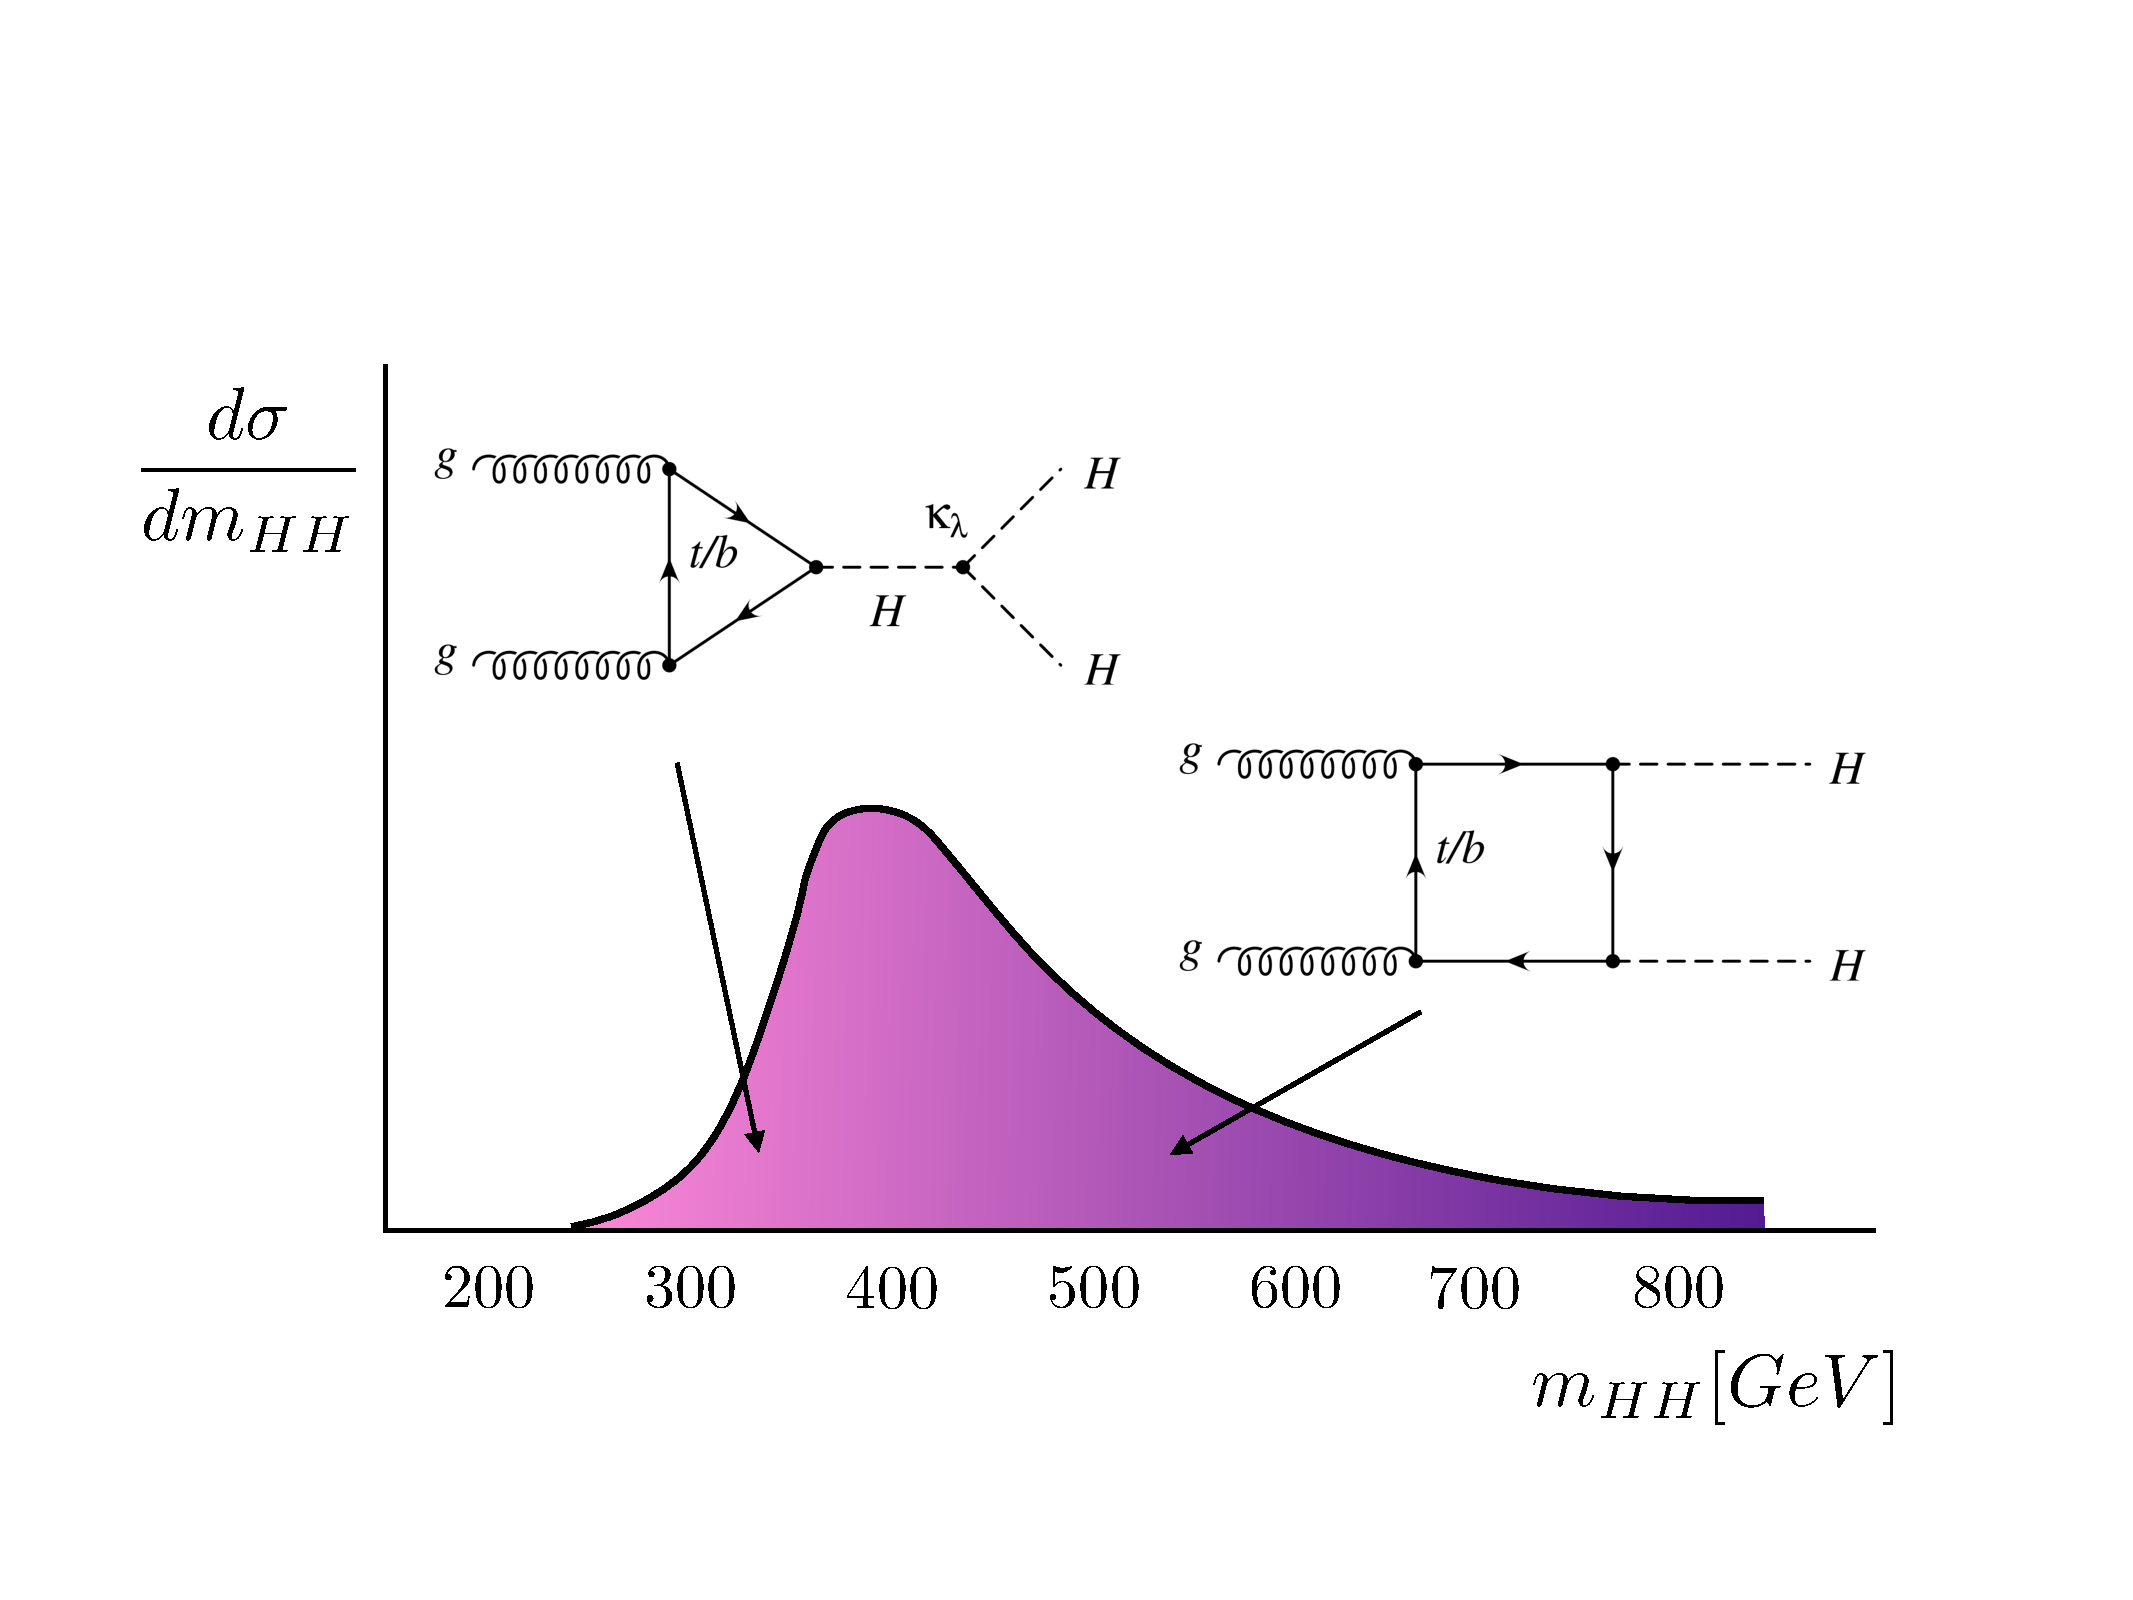
\includegraphics[width=0.7\textwidth]{Part1/Img/mHHSketch.pdf}}
%\end{figure}

\begin{figure}
    \begin{overprint}
    \onslide<1>\centering\fcolorbox{HHred}{HHwhite2}{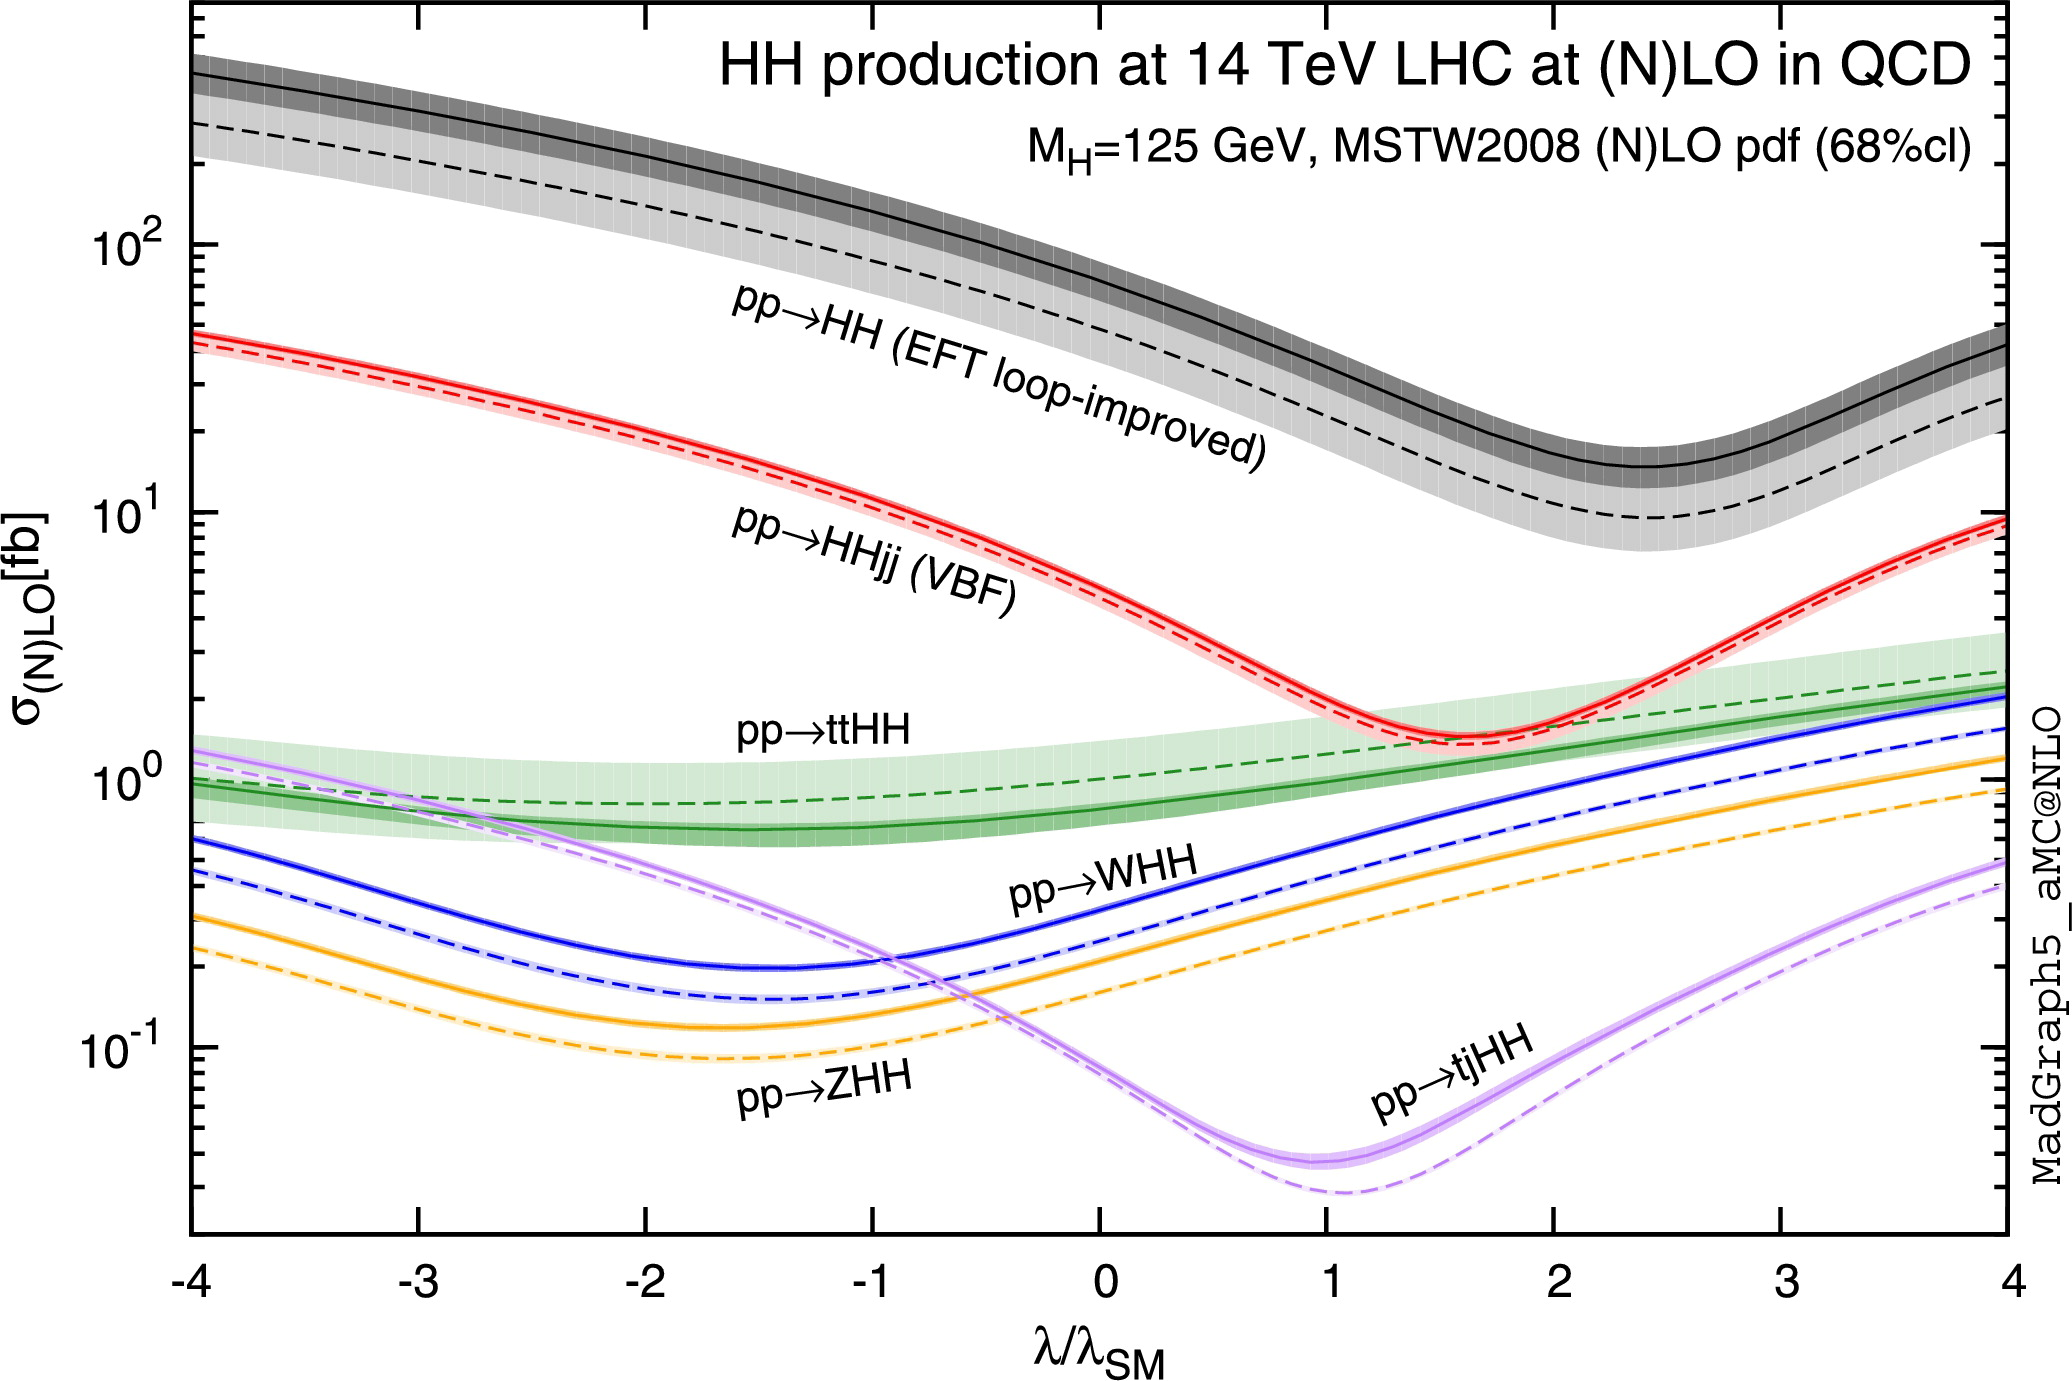
\includegraphics[width=1\textwidth]{Part1/Img/HH_xsec_lambda.jpg}}
    \onslide<2->\centering\fcolorbox{HHturquoise_m}{HHwhite2}{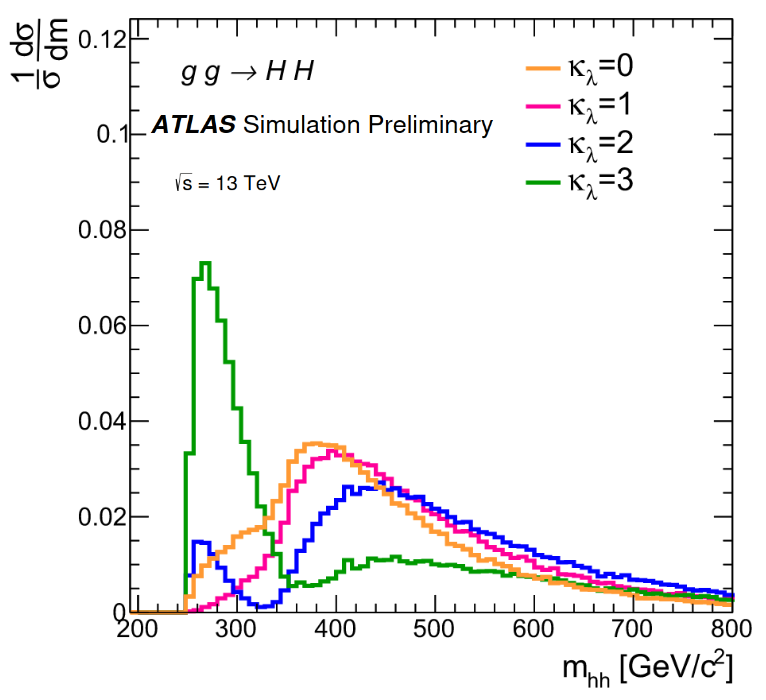
\includegraphics[width=0.9\textwidth]{Part1/Img/mHH.png}}
    \end{overprint}
\end{figure}

\end{columns}
\end{frame}

\begin{frame}{Di-Higgs boson decay modes}
\begin{textblock*}{5cm}(6.75cm, 5.2cm) % {block width} (coords) 
  \textcolor{HHred}{\textbf{$\star$}}
\end{textblock*}

\begin{figure}
    \centering
    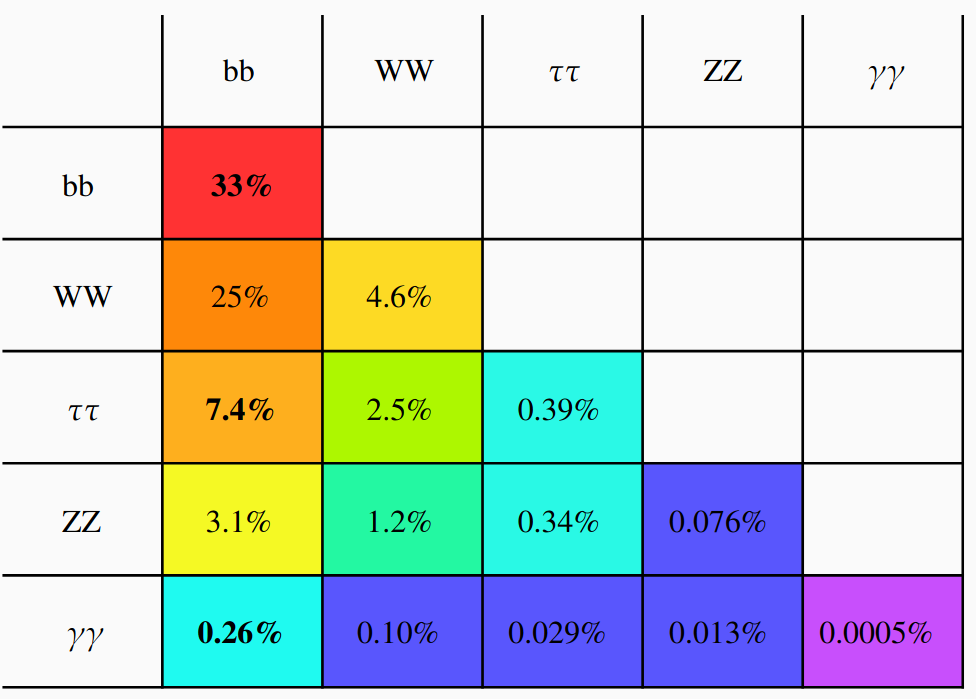
\includegraphics[width=0.43\textwidth]{Part1/Img/HH_decays2.png}
\end{figure}
\pause
\begin{itemize}
    \item \textbf{\textcolor{HHred}{Focusing on H($\to b\bar{b}$)H($\to\gamma\gamma$)}}
    \item Despite low decay rate, competitive channel
    \begin{itemize}
        \item \textbf{High} H$\to b\bar{b}$ branching ratio
        \item \textbf{Excellent} $m_{\gamma\gamma}$ mass resolution $\to$ \textbf{Good signal extraction}
    
    \end{itemize}
\end{itemize}

\end{frame}

\section{Experimental setup}

\begin{frame}{Content}
\label{content}
    \tableofcontents[currentsection]
\end{frame}

\subsection{The Large Hadron Collider}
\begin{frame}{The LHC}
    
\end{frame}

\subsection{The ATLAS detector}
\begin{frame}{The ATLAS detector}

\end{frame}

\subsection{Particles reconstruction}
\begin{frame}{Particles reconstruction}

\end{frame}

\begin{frame}{More about photons}

\end{frame}

\begin{frame}{More about jets}

\end{frame}

\end{document}